\begin{name}
	{\tenchude}
	{\tendethi}
	{\tentruong}
	{\thoigian}
\end{name}
\Opensolutionfile{ansbook}[ans/ansbookDe1]
\TN
\Opensolutionfile{ans}[ans/ansDe1-TN1]
\begin{ex}%[1D6N1-1]%[Dự án đề thi HKII Toán khối 11 NH 23 24-Dot16- Nguyễn Ngọc Huy Trường]%[THPT Chuyên Nguyễn Huệ - Hà Nội]
	Cho $a$ là số thực dương; $\alpha$, $\beta$ là các số thực bất kì. Khẳng định nào sau đây là đúng?
	\choice
	{$a^\alpha + a^\beta = a^{\alpha\beta}$}
	{\True $a^\alpha\cdot a^\beta = a^{\alpha + \beta}$}
	{$a^\alpha\cdot a^\beta = a^{\alpha\beta}$}
	{$a^\alpha + a^\beta = a^{\alpha + \beta}$}
	\loigiai{
	Ta có $a^\alpha\cdot a^\beta = a^{\alpha + \beta}$.
	}
	\end{ex}

\begin{ex}%[1D6N2-2]
Với $a$, $b$ là các số thực dương tùy ý và $a\ne 1$, $\log_{a^5}b$ bằng
\choice
{$5\log_ab$}
{$\dfrac{1}{5}+\log_ab$}
{$5+\log_ab$}
{\True $\dfrac{1}{5}\log_ab$}
\loigiai{
Ta có $\log_{a^5}b=\dfrac{1}{5}\log_ab$.
}
\end{ex}

\begin{ex}%[1D6N3-1]
Hàm số nào dưới đây đồng biến trên tập xác định của nó?
\choice
{\True $y=\left(\sqrt{3}\right)^x$}
{$y=\left(\dfrac{1}{2}\right)^x$}
{$y=\left(\dfrac{2}{3}\right)^x$}
{$y=\left(\dfrac{1}{\pi}\right)^x$}
\loigiai{
Hàm số $y=\left(\sqrt{3}\right)^x$ là hàm số mũ với cơ số $\sqrt{3}>1$ nên đồng biến trên $\mathbb{R}$.
}
\end{ex}

\begin{ex}%[1H8N1-1]
Trong các mệnh đề sau đây, mệnh đề nào đúng?
\choice
{\True Hai đường thẳng phân biệt cùng vuông góc với đường thẳng thứ ba thì có thể vuông góc với nhau}
{Hai đường thẳng phân biệt cùng vuông góc với đường thẳng thứ ba thì song song với nhau}
{Hai đường thẳng phân biệt cùng vuông góc với đường thẳng thứ ba thì vuông góc với nhau}
{Hai đường thẳng phân biệt cùng vuông góc với đường thẳng thứ ba thì hoặc song song với nhau hoặc vuông góc với nhau}
\loigiai{
Hai đường thẳng phân biệt cùng vuông góc với đường thẳng thứ ba thì có thể vuông góc với nhau.
}
\end{ex}

\begin{ex}%[10-11-EX-GK2-2425]%[Trần Như Cang]%[1H8N2-1]
Trong không gian, cho điểm $O$ và đường thẳng $d$. Qua điểm $O$ có bao nhiêu mặt phẳng vuông góc với đường thẳng $d$?
\choice
{$2$}
{Vô số}
{$3$}
{\True $1$}
\loigiai{Chỉ có duy nhất một mặt phẳng đi qua một điểm và vuông góc với một đường thẳng cho trước.}
\end{ex}

\begin{ex}%[1H8N4-1]
	Cho hình hộp chữ nhật $ABCD.A'B'C'D'$. Khẳng định nào sau đây sai?
	\choice
	{Hình hộp có $6$ mặt là $6$ hình chữ nhật}
	{\True $\left( ACC'A' \right)\perp \left( BDD'B' \right)$}
	{Hình hộp có bốn đường chéo bằng nhau}
	{Tồn tại điểm cách đều tám đỉnh của hình hộp}
	\loigiai{
	\immini{
	Ta có $ABCD$ là hình chữ nhật nên $AC$ và $BD$ không vuông góc với nhau\\
	$\Rightarrow $ Hai mặt phẳng $\left( ACC'A' \right)$ và $\left( BDD'B' \right)$ không vuông góc với nhau.}
	{
	\begin{tikzpicture}[line join=round,line cap=round,line width=.6pt,font=\footnotesize,scale=1]
	\coordinate[label=below left:$B$] (B) at (0,0);
	\coordinate[label=above left:$A$] (A) at (1,.8);
	\coordinate[label=below right:$C$] (C) at (5,0);
	\coordinate[label=above right:$D$] (D) at ($(C)-(B)+(A)$);
	\coordinate[label=above left:$A'$] (A1) at ($(A)+(90:4)$);
	\coordinate[label=left:$B'$] (B1) at ($(B)-(A)+(A1)$);
	\coordinate[label=below right:$C'$] (C1) at ($(C)-(A)+(A1)$);
	\coordinate[label=above right:$D'$] (D1) at ($(D)-(A)+(A1)$);
	\draw (B1)--(B)--(C)--(D)--(D1)--(A1)--(B1)--(C1)--(D1) (C)--(C1);
	\draw[dashed] (A)--(D) (A1)--(A)--(B);
	\fill (A)circle(2pt) (B)circle(2pt) (C)circle(2pt) (D)circle(2pt) (A1)circle(2pt) (B1)circle(2pt) (C1)circle(2pt) (D1)circle(2pt);
	\end{tikzpicture}
	
	}
	}
	\end{ex}

\begin{ex}%[1H8N6-1]
\immini{	Cho hình chóp $S.ABC$ có $\triangle ABC$ vuông tại $B$ và $SA\perp \left(ABC\right)$. Góc giữa đường thẳng $SC$ và mặt phẳng $\left(SAB\right)$ là góc nào sau đây?
\choice
{$\widehat{SAC}$}
{$\widehat{CSA}$}
{\True $\widehat{CSB}$}
{$\widehat{SCB}$}
}{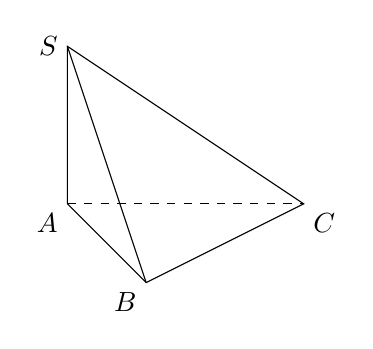
\begin{tikzpicture}
\draw (0,0)--(1,-1)--(3,0)--(0,2)--cycle;
\draw[dashed] (0,0)--(3,0);
\draw (0,2)--(1,-1);
\node[below left] at (0,0) {$A$} ;
\node[below left]at (1,-1) {$B$} ;
\node[below right]at (3,0) {$C$} ;
\node[left]at (0,2) {$S$} ;
\end{tikzpicture}}
\loigiai{ Ta có $\heva{&SA \perp BC\\ &AB \perp BC} \Rightarrow BC \perp (SAB)$.\\
Do dó $SB$ là hình chiếu vuông góc của $SC$ lên mặt phẳng $(SAB)$.\\
Vậy $(SC,(SAB))=(SC,SB)=\widehat{CSB}$.
}
\end{ex}

\begin{ex}.%[1H8N7-1]
Cho khối chóp có diện tích đáy $B$ và chiều cao $h$. Thể tích $V$ của khối chóp đã cho được tính theo công thức nào dưới đây?
\choice
{\True $V=\dfrac{1}{3}Bh$}
{$V=Bh$}
{$V=\dfrac{4}{3}Bh$}
{$V=\dfrac{1}{2}Bh$}
\loigiai{
Công thức thể tích khối chóp là $V=\dfrac{1}{3}Bh$.}
\end{ex}

\begin{ex}%[1D9N1-1]%[Dự án đề kiểm tra Toán 11 GHKII NH23-24- Huỳnh Xuân Tín]%[THPT Hoàng Văn Thụ- Hà Nội]
Cho $A$, $ B$ là hai biến cố độc lập và $\mathrm{P}(A)=0{,}4$; $ \mathrm{P}(AB)=0{,}3$. Xác suất của biến cố $B$ là
\choice
{\True $\mathrm{P}(B)=0{,}75$}
{$\mathrm{P}(B)=0{,}5$}
{$\mathrm{P}(B)=0{,}12$}
{$\mathrm{P}(B)=0{,}2$}
\loigiai{Vì $A$, $ B$ là hai biến cố độc lập nên $\mathrm{P}(AB)=\mathrm{P}(A)\cdot\mathrm{P}(B)$.\\
Khi đó $\mathrm{P}(B)=\dfrac{\mathrm{P}(AB)}{\mathrm{P}(A)}=\dfrac{0{,}3}{0{,}4}=0{,}75$. }
\end{ex}

\begin{ex}%[1D9N2-1]
Cho $A$ và $B$ là hai biến cố xung khắc. Chọn phát biểu đúng:
\choice
{\True $\mathrm{P}(A \cup B) = \mathrm{P}(A) + \mathrm{P}(B)$}
{$\mathrm{P}(A \cup B) = \mathrm{P}(A) - \mathrm{P}(B)$}
{$\mathrm{P}(A \cap B) = \mathrm{P}(A) + \mathrm{P}(B)$}
{$\mathrm{P}(A \cap B) = \mathrm{P}(A) - \mathrm{P}(B)$}
\loigiai{
Vì $A$ và $B$ là hai biến cố xung khắc nên $\mathrm{P}(AB) = 0$.
Do đó, ta có
\[\mathrm{P}(A \cup B) = \mathrm{P}(A) + \mathrm{P}(B).\]
}
\end{ex}

\begin{ex}%[1D7N1-1]%[Dự án đề thi HKII Toán khối 11 NH 23 24-Dot16- Nguyễn Ngọc Huy Trường]%[THPT Chuyên Nguyễn Huệ - Hà Nội]
Hàm số $y=f(x)$ có đạo hàm tại $x=2$ là $f'(2)$. Khẳng định nào sau đây là đúng?
\choice
{$f'(2) = \lim\limits_{x\to 2}\dfrac{f(x)+f(2)}{x-2}$}
{$f'(2) = \lim\limits_{x\to 2}\dfrac{f(x)+f(2)}{x+2}$}
{\True $f'(2) = \lim\limits_{x\to 2}\dfrac{f(x)-f(2)}{x-2}$}
{$f'(2) = \lim\limits_{x\to 2}\dfrac{f(x)-f(2)}{x+2}$}
\loigiai{
Ta có $f'(2) = \lim\limits_{x\to 2}\dfrac{f(x)-f(2)}{x-2}$.
}
\end{ex}

\begin{ex}%[1D7N3-1]  :
Đạo hàm cấp hai của hàm số $y=\cos^2x$ là
\choice
{\True  $ y'' =-2\cos 2x$}
{$ y'' =-2\sin 2x$}
{$ y'' =2\cos 2x$}
{$ y'' =2\sin 2x$}
\loigiai{
$y=\cos^2x \Rightarrow y'=2\cos x (-\sin x)=-\sin 2x $, $ y'' =-2\cos 2x$.
}
\end{ex}
\Closesolutionfile{ans}

\TNTF
\Opensolutionfile{ans}[ans/ansDe1-TN2]
\begin{ex}
Cho hàm số $y=f(x)=ax^2-3x+2$ với $a \ne 0$ có $f'(1)=1$ và đồ thị $(C)$.
\choiceTF
{\True $\lim\limits_{x\to 1} \dfrac{f(x)-f(1)}{x-1}=1$}
{$f'(x)=2ax+1$}
{\True Phương trình tiếp tuyến của $(C)$ tại có hoành độ bằng $1$ là $y=x$}
{Cho $g(x)=f(x^2+1)$, khi đó $g'(1)=0$}
\loigiai{
\begin{itemchoice}
\itemch \textbf{Đúng.} Ta có $\lim\limits_{x\to 1} \dfrac{f(x)-f(1)}{x-1}=f'(1)=1$.
\itemch \textbf{Sai.} Ta có $f'(x)=2ax-3$.
\itemch \textbf{Đúng.} $f'(1)=2a-3=1 \Rightarrow a=2$. Do đó $f(1)=2-3+2=1$.\\
Phương trình tiếp tuyến tại $M(1;1)$ là $y=f'(1)(x-1)+f(1) \Leftrightarrow y=1(x-1)+1 \Leftrightarrow y=x$.
\itemch \textbf{Sai.} Ta có $g'(x)=f'(x^2+1)\cdot (x^2+1)'=f'(x^2+1)\cdot 2x$.\\
Với $x=1 \Rightarrow g'(1)=f'(2)\cdot 2=5\cdot 2=10$.
\end{itemchoice}
}
\end{ex}

\begin{ex}%[1D7H2-1]%[1D7H2-5]%[tex hóa đề ck2 - form 2025 - đợt 2 - Thành Đức Trung]
Cho hàm số $f(x)=x^2-3x+2$ và hàm số $g(x)=2x^3-3x^2+5$. Khi đó
\choiceTF
{\True $f'(x)=2x-3$}
{\True Tính đạo hàm của hàm số $h(x)=\dfrac{f(x)}{g(x)}$ ta được $h'(x)=\dfrac{-2x^4+12x^3-21x^2+22x-15}{(2x^3-3x^2+5)^2}$}
{Hàm số $g(x)$ có đồ thị $(C)$. Khi đó từ điểm $A\left(\dfrac{19}{12};4\right)$ kẻ được $2$ tiếp tuyến tới $(C)$}
{Phương trình $4f'(x)-(2x-5)f'' (x)-x+1=2\sqrt{25-x^2}$ vô nghiệm}
\loigiai
{
\begin{itemchoice}
\itemch Đúng. Vì $f'(x)=(x^2-3x+2)'=2x-3$.
\itemch Đúng. Vì
$\begin{aligned}[t]
h'(x)&=\left(\dfrac{x^2-3x+2}{2x^3-3x^2+5}\right)'\\
&=\dfrac{(2x-3)(2x^3-3x^2+5)-(x^2-3x+2)(6x^2-6x)}{(2x^3-3x^2+5)^2}\\
&=\dfrac{-2x^4+12x^3-21x^2+22x-15}{(2x^3-3x^2+5)^2}.
\end{aligned}$
\itemch Sai. Vì gọi $k$ là hệ số góc của tiếp tuyến đi qua $A\left(\dfrac{19}{12};4\right)$ tới $(C)$.\\
Phương trình tiếp tuyến $(\Delta)$ là $y=k\left(x-\dfrac{19}{12}\right)+4$. \\
$(\Delta)$ tiếp xúc với $(C) \Leftrightarrow \heva{&2x^3-3x^2+5=k\left(x-\dfrac{19}{12}\right)+4 \ \ &&(1)\\&6x^2-6x=k \ \ &&(2)}$ có nghiệm.\\
Thay $k$ từ $(2)$ vào $(1)$ ta được \\
\[\begin{aligned}
& \ 2x^3-3x^2+5=(6x^2-6x)\left(x-\dfrac{19}{12}\right)+4 \\
\Leftrightarrow & \ 4x^3-6x^2+2=(x^2-x)(12x-19) \\
\Leftrightarrow & \ 8x^3-25x^2+19x-2=0 \\
\Leftrightarrow & \ \hoac{&x=1\\&x=2\\&x=\dfrac{1}{8}.}
\end{aligned}\]
Với $x=1 \Rightarrow k=0$, suy ra phương trình tiếp tuyến là
\[y=4.\]
Với $x=2\Rightarrow k=12$, suy ra phương trình tiếp tuyến là
\[y=12\left(x-\dfrac{19}{12}\right)+4 \Leftrightarrow y=12x-15.\]
Với $x=\dfrac{1}{8}\Rightarrow k=-\dfrac{21}{32}$, suy ra phương trình tiếp tuyến là
\[y=-\dfrac{21}{32}\left(x-\dfrac{19}{12}\right)+4 \Leftrightarrow y=-\dfrac{21}{32}x+\dfrac{645}{128}.\]
Vậy từ điểm $A\left(\dfrac{19}{12};4\right)$ kẻ được $3$ tiếp tuyến tới $(C)$.
\itemch Sai. Vì ta có $f'(x)=2x-3 \Rightarrow f'' (x)=2$.\\
Do đó
\[\begin{aligned}
& \ 4f'(x)-(2x-5)f'' (x)-x+1=2\sqrt{25-x^2} \\
\Leftrightarrow & \ 4(2x-3)-2(2x-5)-x+1=2\sqrt{25-x^2} \\
\Leftrightarrow & \ 8x-12-4x+10-x+1=2\sqrt{25-x^2} \\
\Leftrightarrow & \ 3x-1=2\sqrt{25-x^2} \\
\Leftrightarrow & \ \heva{&x\geqslant \dfrac{1}{3}\\&9x^2-6x+1=4(25-x^2)} \\
\Leftrightarrow & \ \heva{&x\geqslant \dfrac{1}{3}\\&9x^2-6x+1=100-4x^2} \\
\Leftrightarrow & \ \heva{&x\geqslant \dfrac{1}{3}\\&13x^2-6x-99=0} \\
\Leftrightarrow & \ \heva{&x\geqslant \dfrac{1}{3}\\&\hoac{&x=3\\&x=-\dfrac{33}{13}}} \\
\Leftrightarrow & \ x=3.
\end{aligned}\]
\end{itemchoice}
}
\end{ex}
\Closesolutionfile{ans}

\TNSA
\Opensolutionfile{ans}[ans/ansDe1-TN3]
\begin{ex}%[Dự án đề kiểm tra Toán 11 HKII NH23-24- Nguyễn Tấn Linh]%[THPT Trần Khai Nguyên - Tp HCM]%[1D6H4-3]
Tìm nghiệm nguyên dương nhỏ nhất của bất phương trình $\left(\dfrac{1}{2}\right)^{x-3}\ge(0,25)^{x-1}$.
\shortans{$1$}
\loigiai{
Ta có
\begin{eqnarray*}
&&\left(\dfrac{1}{2}\right)^{x-3} \ge (0,25)^{x-1}\\
&\Leftrightarrow &\left(\dfrac{1}{2}\right)^{x-3} \ge \left(\dfrac{1}{2}\right) ^{2x-2}\\
&\Leftrightarrow& x-3 \le 2x-2 ~ \left(0<\dfrac12<1\right) \\
&\Leftrightarrow& x \ge -1.
\end{eqnarray*}
Vậy nghiệm nguyên dương nhỏ nhất của bất phương trình là $1$.
}
\end{ex}

\begin{ex}%[Dự án 17 - CK2 NH23-24 - TeamTeXHoa - Nguyễn Sơn Thành]%[1H8H5-4]
	Cho hình chóp tứ giác đều $S.ABCD$  có đáy là hình vuông cạnh $a$, cạnh bên $SA=a\sqrt{2}$. Khi  $a=\sqrt{42}$ thì khoảng cách giữa hai đường thẳng $AB$  và $SC$  bằng bao nhiêu?
	\shortans[0]{$6$}
	\loigiai{
	\begin{center}
	\begin{tikzpicture}[scale=0.7, font=\footnotesize,line join=round, line cap=round, >=stealth]
	\path
	(0:0) coordinate (A)
	(0:5) coordinate (D)
	(-135:2.8) coordinate (B)
	+(D) coordinate (C)
	
	($(B)!0.5!(D)$) coordinate (O)+(90:5) coordinate (S)
	($(C)!0.5!(D)$) coordinate (N)
	($(A)!0.5!(B)$) coordinate (M)
	($(S)!0.6!(N)$) coordinate (I)
	;
	\draw[dashed] (B)--(A)--(D)--(B) (O)--(S)--(A) (A)--(C) (I)--(M)--(N);
	\draw[thick] (S)--(B) (S)--(C) (S)--(D) (C)--(B) (D)--(C) (S)--(N);
	\foreach \x/\g in {A/135,B/180,C/-30,D/0,S/90,O/-90,N/0,M/100,I/0}\draw[fill=white] (\x) circle (.03) +(\g:.3) node{$\x$};
	\end{tikzpicture}
	\end{center}
	Gọi  $O$ là tâm hình vuông $ABCD$. $M$, $N$  lần lượt là trung điểm của $AB$, $CD$.\\ Khi đó $\mathrm{d}\left(AB, CD\right)=\mathrm{d}\left(AB, \left(SCD\right)\right)=\mathrm{d}\left(M, \left(SCD\right)\right)$.\\
	Ta có  $\heva{&CD\bot MN\\&CD\bot SO}\Rightarrow CD\bot \left(SMN\right)\Rightarrow \left(SCD\right)\bot \left(SMN\right)$ mà  $\left(SCD\right)\cap \left(SMN\right)=SN$.\\
	Do đó, trong $\left(SMN\right)$  kẻ $MI\bot SN$, $\left(I\in SN\right)$  thì  $MI \bot \left(SCD\right)\Rightarrow \mathrm{d}\left(M, \left(SCD\right)\right)=MI$.\\
	Xét tam giác $SAC$  có $SA=SC=AC=a\sqrt{2}$  nên $\Delta SAC$  đều, do đó $SO=\dfrac{a\sqrt{6}}{2}$.\\
	Ta lại có  $MI\cdot SN=SO\cdot MN \Rightarrow MI=\dfrac{SO\cdot MN}{SN}=\dfrac{\dfrac{a\sqrt{6}}{2}\cdot a}{\sqrt{\left(a\sqrt{2}\right)^2-\left(\dfrac{a}{2}\right)^2}}=\dfrac{a\sqrt{42}}{7}$.\\
	Vậy  $\mathrm{d}\left(AB, CD\right)=\dfrac{a\sqrt{42}}{7} \xrightarrow{a=\sqrt{42}} \mathrm{d}\left(AB, CD\right)=6$.
	}
	\end{ex}

\begin{ex}%[1D9V2-4]%[Dự án - 2025_TLDT Toán 11]%[Nguyễn Tiến Liên]
Cho hai biến cố độc lập $A$ và $B$. Biết $\mathrm{P}(A)=\dfrac{1}{4}$, $\mathrm{P}( A\cup B )=\dfrac{1}{2}$. Khi đó $\mathrm{P}(B)$ bằng bao nhiêu (\textit{làm tròn kết quả đến hàng phần chục})?
\shortans{$0{,}3$}
\loigiai{
Theo công thức xác suất của biến cố hợp, ta có $\mathrm{P}(A\cup B)=\mathrm{P}(A)+\mathrm{P}(B)-\mathrm{P}(AB)$.\\
Tuy nhiên do $A;B$ là hai biến cố độc lập nên $\mathrm{P}(A\cdot B)=\mathrm{P}(A)\cdot \mathrm{P}(B)$.\\
Vậy ta có \\
$\mathrm{P}(A\cup B)=\mathrm{P}(A)+\mathrm{P}(B)-\mathrm{P}(A)\cdot \mathrm{P}(B)\Leftrightarrow \dfrac{1}{2}=\dfrac{1}{4}+\mathrm{P}(B )-\dfrac{1}{4}\cdot \mathrm{P}(B)\Rightarrow \mathrm{P}(B)=\dfrac{1}{3}=0{,}3$.
}
\end{ex}

\begin{ex}%[1D7V2-8]
	Một chất điểm chuyển động có quãng đường được cho bởi phương trình $S(t)=\dfrac{1}{4} t^4-t^3+\dfrac{7}{2} t^2+12t$, trong đó $t > 0$ với $t$ được tính bằng giây $(s)$ và $S$ được tính bằng mét $(m)$. Hỏi tại thời điểm gia tốc của vật đạt giá trị nhỏ nhất thì vận tốc của vật bằng bao nhiêu?
	\shortans[0]{$17$}
	\loigiai{
	Phương trình vận tốc của chuyển động $v(t)=S'(t)=t^3-3t^2+7t+12$.\\
	Phương trình gia tốc của chuyển động $a(t)=v'(t)=3t^2-6t+7$.\\
	Ta có $a(t)=3t^2-6t+7=3\left(t-1\right)^2+4\ge 4$ với mọi $t$.\\
	Dấu \lq\lq =\rq\rq  xảy ra khi $t=1$.\\
	Khi đó, vận tốc của chuyển động là $v(1)=17$ (m/s).
	}
\end{ex}
\Closesolutionfile{ans}

\TL
\begin{ex}%[1D7H2-1]%[TLD Toán T11-Toán từ Tâm]%[Dương Công Tạo]
Tính đạo hàm các hàm số sau
\begin{enumEX}{2}
\item $f(x)=\left(1-x^3 \right)^5$.
\item $f(x)=\dfrac{3x+5}{-1+2x}$.
\end{enumEX}
\loigiai{
\begin{enumerate}
\item $f(x)=\left(1-x^3 \right)^5$.\\
Ta có $f'(x)=5\left(1-x^3 \right)^4 \left(1-x^3 \right)'=-15x^2 \left(1-x^3 \right)^4$.
\item $f(x)=\dfrac{3x+5}{-1+2x}$.\\
Ta có \begin{eqnarray*}
f'(x)&=&\dfrac{(3x+5)'\cdot(2x-1)-(3x+5)(2x-1)'}{(2x-1)^2}\\
&=&\dfrac{3(2x-1)-2(3x+5)}{(2x-1)^2}\\
&=&\dfrac{-13}{(2x-1)^2}.
\end{eqnarray*}
\end{enumerate}
}
\end{ex}

\begin{ex}%[1H8V5-4]
Cho hình chóp $S.ABCD$ có đáy là hình vuông cạnh bằng $2$, $SA$ vuông góc với mặt phẳng đáy và $SA=\sqrt{5}$. Gọi $M$, $N$ là trung điểm của $SA$ và $CD$. Tính khoảng cách giữa hai đường thẳng $MN$ và $SC$.
\loigiai{\immini{Gọi $O$ là tâm của hình vuông $ABCD$.\\
Ta có $OM$ là đường trung bình của tam giác $SAC$ nên $OM\parallel SC$.\\
Mặt khác ta có $\heva{&OM\subset(OMN)\\&SC\not\subset(OMN)}\Rightarrow SC\parallel(OMN)$.\\
Mà $MN\subset(OMN)$ nên
\[\mathrm{d}(MN,SC)=\mathrm{d}(SC,(OMN))=\mathrm{d}(C,(OMN)).\]
Do $AC$ cắt $(OMN)$ tại $O$ nên}
{\begin{tikzpicture}[>=stealth,line join=round,line cap=round,font=\footnotesize,scale=0.5]
\path (0,0) coordinate (A)
(-2.5,-1.4) coordinate (B)
(6,0) coordinate (D)
($(B)+(D)-(A)$) coordinate (C)
($(A)!0.5!(C)$) coordinate (O)
($(A)+(0,6)$)coordinate (S)
($(A)!0.5!(S)$) coordinate (M)
($(A)!0.5!(B)$) coordinate (P)
($(C)!0.5!(D)$) coordinate (N)
($(M)!0.65!(P)$) coordinate (H)
;
\draw (S)--(B)--(C)--(S)--(D)--(C);
\draw[dashed] (S)--(A)--(B)--(D)--(A)--(C) (A)--(H) (M)--(P)--(N)--(M)--(O);
\foreach \p / \r in {A/45,B/-135,C/-45,S/90,M/135,O/-90,D/45,N/-45,H/135,P/135}
\fill (\p) circle (1.2pt) node[shift={(\r:2.5mm)}]{$\p$};
\end{tikzpicture}}
\[\dfrac{\mathrm{d}(C,(OMN))}{\mathrm{d}(A,(OMN))}=\dfrac{OC}{OA}=1\Rightarrow\mathrm{d}(C,(OMN))=\mathrm{d}(A,(OMN)).\]
Gọi $P$ là trung điểm của $AB$, ta có $(OMN)$ cũng chính là $(MNP)$.\\
Ta có $\heva{&NP\perp AB\\&NP\perp SA}\Rightarrow NP\perp(SAB)$.\\
Do $NP\subset(MNP)$ nên $(MNP)\perp(SAB)$ theo giao tuyến $MP$.\\
Gọi $H$ là hình chiếu vuông góc của $A$ lên $MP$ trong $(SAB)$, suy ra $AH\perp(MNP)$ tại $H$.\\
Tam giác $AMP$ có $\dfrac{1}{AH^2}=\dfrac{1}{AP^2}+\dfrac{1}{AM^2}=\dfrac{9}{5}\Rightarrow AH=\dfrac{\sqrt{5}}{3}$.\\
Vậy $\mathrm{d}(MN,SC)=\mathrm{d}(A,(MNP))=AH=\dfrac{\sqrt{5}}{3}$.}
\end{ex}
\begin{ex}%[VDC8-ThanDucMinh]%[1D2G2-6]
	Một trường phổ thông có $15$ giáo viên Toán trong đó có $5$ nữ, $10$ giáo viên Lý trong đó có $4$ nữ. Chọn ngẫu nhiên $5$ giáo viên. Tính xác suất trong $5$ giáo viên được chọn có cả Toán và Lý, có cả nam và nữ.
	% \choice
	% {$\dfrac{3051}{3542}$}
	% {$\dfrac{120}{253}$}
	% {\True $\dfrac{652}{759}$}
	% {$\dfrac{652}{579}$}
	\loigiai{
		Số phần tử của không gian mẫu là $\left|\Omega\right|=C_{25}^5=53130$.
		\begin{itemize}
			\item Số cách chọn $5$ giáo viên có cả Toán và Lý là $C_{25}^5-C_{15}^5-C_{10}^5=49875$.
			\item Số cách chọn $5$ giáo viên nam có cả Toán và Lý là  $C_{16}^5-C_{10}^5-C_6^5=4110$.
			\item Số cách chọn $5$ giáo viên nữ có cả Toán và Lý là $C_9^5-C_5^5=125$.
		\end{itemize}
		Gọi $A$ là biến cố \lq \lq Chọn $5$ giáo viên Toán, trong đó có cả Toán và Lý, có cả nam và nữ.\rq \rq\\
		Ta có: $\left|\Omega_A\right|=45640$.\\
		Xác suất cần tìm là $P\left(A\right)=\dfrac{\left|\Omega_A\right|}{\left|\Omega\right|}=\dfrac{45640}{53130}=\dfrac{652}{759}$.
	}
\end{ex}
\Closesolutionfile{ansbook}
% \HetDe
% \label{De1}
% %
% \cleardoublepage
% \setcounter{page}{1}
% \rfoot{Trang \thepage/\pageref{DA1} - Đáp án trắc nghiệm Đề 1}
% \begin{center}
% 	\bfseries ĐÁP ÁN TRẮC NGHIỆM ĐỀ 1
% \end{center}

% \inputansbox{10}{ans/ansDe1-TN1}
% \inputansbox[3]{2}{ans/ansDe1-TN2}
% \inputansbox{3}{ans/ansDe1-TN3}
% \label{DA1}
% %
